\documentclass[11pt, a4paper]{article}

% Packages for math, formatting, and graphics
\usepackage[utf8]{inputenc}
\usepackage{amsmath, amsfonts, amssymb}
\usepackage{geometry}
\usepackage{enumitem}
\usepackage{hyperref}
\usepackage{tikz}

% TikZ libraries for advanced drawing features
\usetikzlibrary{patterns, arrows.meta, positioning}

% Set page margins
\geometry{
    top=1.2in,
    bottom=1.2in,
    left=1in,
    right=1in
}

% Remove paragraph indentation
\setlength{\parindent}{0pt}

\begin{document}

% Header Section
\begin{center}
    CE 512 Finite Element Method
\end{center}
\vspace{-0.6cm}
Homework 3 \hfill 2026 Spring \hfill \null \\
Due Date: 23.03.2026 -- 01:00 \hfill (upload to \url{https://cloud-lms.iyte.edu.tr} )

\vspace{0.8cm}

% Questions Section
\begin{enumerate}[label=\arabic*., leftmargin=*]
    \item Read pages 81-88, Cook (Section on ``Comment on the Rayleigh-Ritz Method ...'')

    \vspace{0.3cm}
    The figure below shows a similar problem as discussed in the Lecture. Here, a load, P, is applied at the member mid-length, and at the right end. Find the formulation of the displacement field (i.e. find the constants $a_i$.)

    \vspace{0.2cm}
    \begin{enumerate}[label=\alph*)]
        \item Let $u(x) = a_2 x^2$
        \item Let $u(x) = a_2 x^2 + a_3 x^3$
        \item Plot the displacement fields calculated in a) and b) onto a single graph.
        \item Plot the stress variation for a) and b) onto a single graph.
    \end{enumerate}

    \vspace{0.6cm}
    % TikZ Diagram
    \begin{center}
        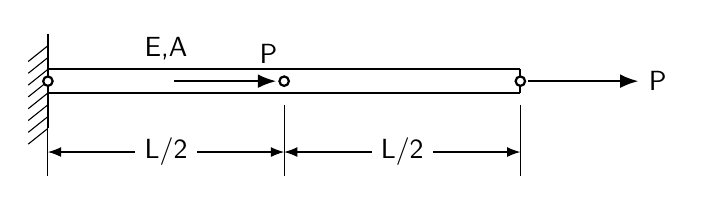
\begin{tikzpicture}[>=Latex, font=\sffamily]
            
            % 1. Fixed Support (Left Wall)
            \draw[thick] (0, 0.6) -- (0, -0.6);
            \foreach \y in {-0.6, -0.45, ..., 0.6} {
                \draw (0,\y) -- (-0.25,\y-0.2);
            }

            % 2. 1-D Bar Element (Hollow Profile)
            \draw[thick] (0, 0.15) -- (6, 0.15);
            \draw[thick] (0, -0.15) -- (6, -0.15);
            \draw[thick] (6, 0.15) -- (6, -0.15);

            % Material/Section Properties
            \node[above] at (1.5, 0.15) {E,A};

            % 3. Applied Loads (Vectors)
            % Mid-length load P
            \draw[thick, ->] (1.6, 0) -- (2.9, 0);
            \node[above] at (2.8, 0.1) {P};

            % Right end load P
            \draw[thick, ->] (6.1, 0) -- (7.5, 0) node[right] {P};

            % 4. Finite Element Nodes (Academic style white-filled points)
            \filldraw[fill=white, draw=black, thick] (0,0) circle (0.06);
            \filldraw[fill=white, draw=black, thick] (3,0) circle (0.06);
            \filldraw[fill=white, draw=black, thick] (6,0) circle (0.06);

            % 5. Dimensions
            % Vertical boundary projection lines
            \draw (0, -0.3) -- (0, -1.2);
            \draw (3, -0.3) -- (3, -1.2);
            \draw (6, -0.3) -- (6, -1.2);

            % Horizontal dimension arrows and labels
            \draw[<->] (0, -0.9) -- (3, -0.9) node[midway, fill=white] {L/2};
            \draw[<->] (3, -0.9) -- (6, -0.9) node[midway, fill=white] {L/2};
            
        \end{tikzpicture}

        \vspace{0.3cm}
        \textit{Figure : 1-D bar element}
    \end{center}

    \vspace{0.6cm}
    \item Reconsider the last lecture with the rectangular finite element of size 2a by 2b. Derive the displacement, u(s,t) in terms of the interpolation functions by starting from the field approximation (as done in class).
    
    \vspace{0.2cm}
    The aim of this duty is to become accustomed to the equations!

\end{enumerate}

\vspace{0.5cm}
As usual, discuss your results.

\end{document}